\documentclass[11pt]{article}

%\usepackage{sectsty}
\usepackage{siunitx}
\usepackage{tabularx}
\usepackage{float}
\usepackage{graphicx}
\usepackage{mathrsfs}
\usepackage{subcaption}
\usepackage{hyperref}
\usepackage{url}
\usepackage{csquotes}
\usepackage{verbatim}
\usepackage{cite}
\usepackage{stfloats}
\usepackage{textcomp}
\usepackage{algorithm}
\usepackage{algorithmic}
\usepackage{amsmath, amsfonts}
\usepackage{cmsrb}
\usepackage[serbian]{babel}

% Margins
\topmargin=-0.45in
\evensidemargin=0in
\oddsidemargin=0in
\textwidth=6.5in
\textheight=9.0in
\headsep=0.25in

\title{MCP3651 based voltmeter module}

\begin{document}

\maketitle
\pagebreak
\tableofcontents
\pagebreak



\section{Resolution}
MCP3651 ADC has a resolution of 24 bits, however, the 7 ppm max 
INL limits this multimeters count to 146000, just shy of 5.5 digit.

Keeping drift in 1 PPM range, 3 uV drift is acceptable over the 
temperature range.

\subsection{Input current noise limit}
Since for input ranges greater then Vcc the input voltage is feed through
a 10 MOhm divider, input currents noise contribution is:

\section{Input amplifier}

\subsection{NCS21802}
NCS21802 has 450 \si{\femto \ampere \sqrt{\hertz}}, meaning at input divider
resistance (around 12 kOhm), voltage noise generated is \si{5.4 nV/\sqrt{Hz}}.

The input voltage noise is \si{54 nV/\sqrt{Hz}}, so total noise at the input
is: 

\begin{equation}
  e_n = \sqrt{ 42^2 + 5.4^2} nV/Hz = 54.3 nV/Hz
  \label{eq:NCS218xx input noise}
\end{equation}

If we want 500 updates a second, setting the bandwidth to 1000 Hz admits 
1716 nVrms, or 10.3 uVpp of noise.
Reducing the BW to 4 Hz, 0.6 uVpp.

With the proposed 10 Meg, 12.5 k divider, worst case scenario is 3V input voltage,
yealding 3.75 mV across the input divider. In this case, noise reduces the 
voltmeter resolution to 500 counts.


Averaging may improve this noise, but this is garantied to 

\section{Power supply}

\subsection{Expected load}
\subsection{Revision 1}



\section{Mounting holes}
4 mounting posts are spaced in a 80 mm by 40 mm rectangle. Plastic post 
hole width is about 2.5 mm, but to allow for a self tapping screw, the PCB 
hole must be M3.

\begin{figure}[H]
  \centering 
  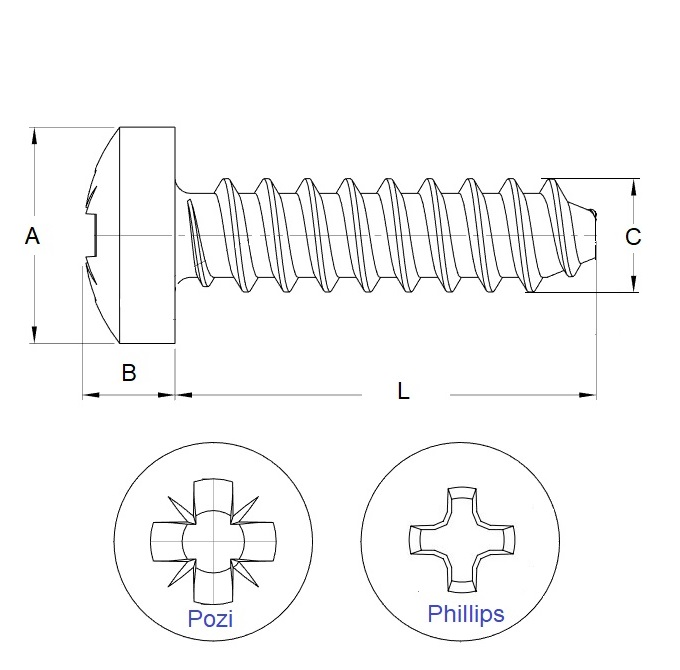
\includegraphics[scale=0.4]{"./figs/screw_sizez.jpg"}
\end{figure}

Apropriate screw is has a B of 2 mm, L of 6 mm, A of 5 mm and C of 3 mm. 

\section{Input connectors}

\subsection{PCB mount connector}

\begin{figure}[H]
  \centering 
  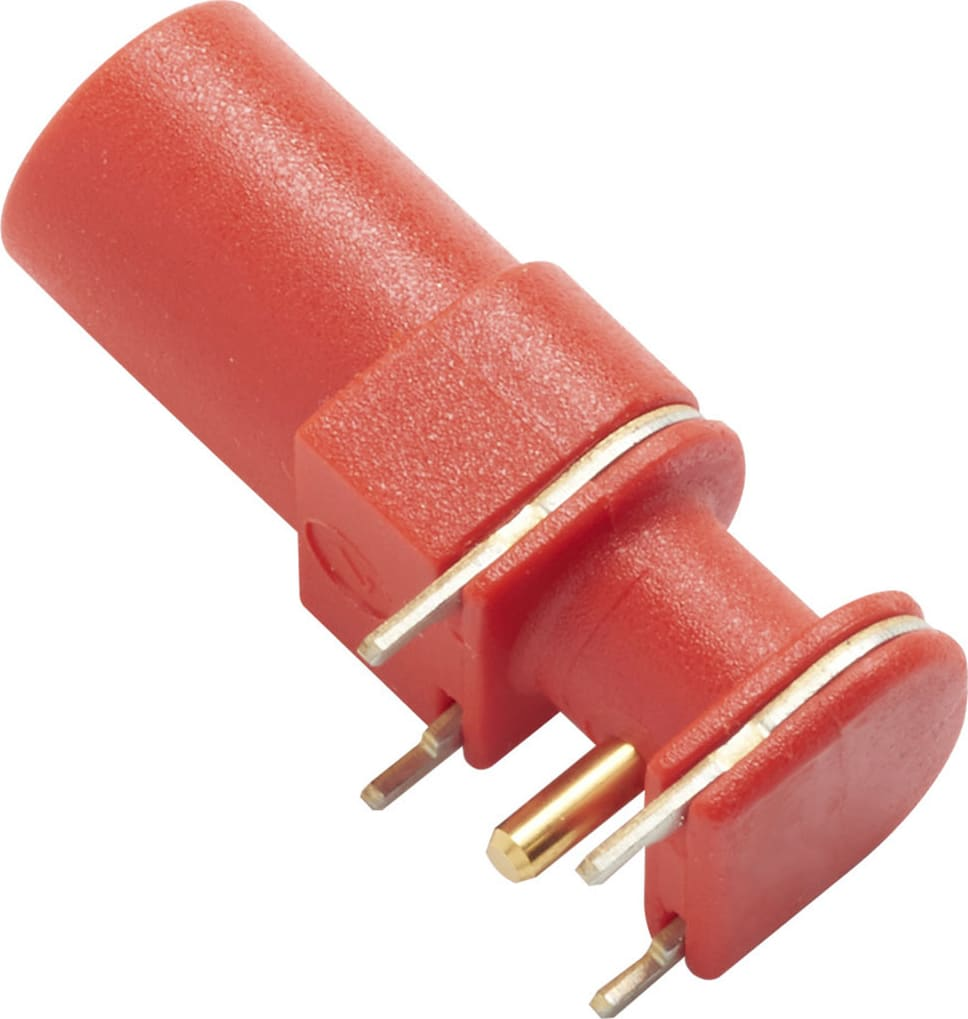
\includegraphics[scale=0.1]{"./figs/pomona.jpg"}
\end{figure}



\href{https://www.mouser.co.uk/ProductDetail/Pomona-Electronics/73099-2?qs=B6kkDfuK7%2FA6DpEPKtHqWw%3D%3D}{Pomona connector} 
  cost around 8 EUR.


\subsection{Panel mount}

\section{Charging connector}
\subsection{Panel mount USB C}

\href{https://www.aliexpress.com/item/1005005795420370.html?spm=a2g0o.detail.pcDetailTopMoreOtherSeller.8.7952vy1gvy1gDZ&gps-id=pcDetailTopMoreOtherSeller&scm=1007.40000.327270.0&scm_id=1007.40000.327270.0&scm-url=1007.40000.327270.0&pvid=2700dcaa-0eb6-4b0e-88eb-943a58278a62&_t=gps-id:pcDetailTopMoreOtherSeller,scm-url:1007.40000.327270.0,pvid:2700dcaa-0eb6-4b0e-88eb-943a58278a62,tpp_buckets:668%232846%238115%232000&pdp_npi=4%40dis%21RSD%2122.34%2118.09%21%21%210.21%210.17%21%402101ef5e17281249438301346ebeab%2112000034381437374%21rec%21SRB%21%21ABXZ&utparam-url=scene%3ApcDetailTopMoreOtherSeller%7Cquery_from%3A}{Aliexpress panel mount USB C connector}
cost around 1.2 EUR per 10 qty.\\

This connector may not have the required resistors in order to negociate 
current demand

\href{https://www.kupujemprodajem.com/elektronika-i-komponente/moduli-za-samoizgradnju/usb-c-konektor-za-montazu/oglas/149804414?filterId=4441321394}{Kupujemprodajem konektor}

\section{Input divider}
\subsection{Resistance divider}
With single sided input impedance of 4 Meg and a required attenuation of 1:400, total
impedance from opamp input to gnd must be:

\begin{equation}
  R_{in} = \frac{4\ \si{\mega \ohm}}{399} = 10.025\ \si{\kilo \ohm}
  \label{eq:res_to_gnd}
\end{equation}

Total resistance to ground is a parallel connection of the dividing resistor,
10 \si{\mega \ohm} input offset trim pot and 10 \si{\mega \ohm} opamp input resistance.

Dividing resistor value should then equal:

\begin{equation}
  R_{div} = \frac{5 \si{\mega \ohm} \cdot 
  10.025 \si{\kilo \ohm}}{5 \si{\mega \ohm} - 10.025 \si{\kilo \ohm}} = 
  10.045 \si{\ohm}
  \label{eq:input_divider}
\end{equation}

Placing a 0.1\% resistor (10.010 \si{\kilo \ohm} max), trim pot should be around 
50 \si{\ohm}.

\subsection{Capacitance divider}
4 series 10 \si{\pico \farad } capacitors yield total 2.5 \si{\pico \farad } with a 
tolerance of 5\%. In order to achieve 1:400 attenuation, total capacitance on the 
buffers input pin should be 997.5 pF. If we account for the 5\% tolerance, 
total capacitance should be trimmable in the range for 947.62 pF to 1047.4 pF.

\href{https://www.analog.com/media/en/technical-documentation/data-sheets/AD8038_8039.pdf}{AD8039}
features a typical input capacitance of 2 pF and thus should not significantly 
impact the total capacitance.


\subsubsection{Trim potenciometers}
Available trimmable capacitor has a capacitance range from 8 pF to 50 pF, not 
enough to account for the 5\% capacitor tolerance.

These trim capacitors are expensive (5 EUR per 1 qty) and are only single turn,
limiting trim accuracy. 


\subsubsection{Varicap trimming}
In order to allow for auto-calibration, input capacitance needs to be control
voltage dependant. To achieve this, a varicap diode may be used.

This component can be trimmed manually, using a trim potentiometer.

Since varicap add a voltage dependant capacitance value, total capacitance before
the adding the varicap needs to be less then the total capacitance required. 

As 5\% capacitors are used, fixed capacitors used should equal:

\begin{equation}
  C_{placed} = \frac{C_{req}}{1.05} - C_{varicap\ min}
  \label{eq:}
\end{equation}

Parallel connection of 2 470 pF yield capacitance in the range of 893 pF to 987 pF.

Since the capacitance change required is 10\% of required capacitance, varicap 
capacitance change in the available control voltage range (0 V to 5V) must be around
100 pF.\\

Diode selection:
\begin{itemize}
  \item Cheaper varicap diode is \href{https://eu.mouser.com/ProductDetail/Toshiba/1SV324TPH3F?qs=EEns8I54Y6DPMP6VMy8m2w%3D%3D}{toshibas}
  at 0.26 EUR per 10 qty. 

  \item Better documented varicap diode is \href{https://eu.mouser.com/ProductDetail/Skyworks-Solutions-Inc/SMV1255-079LF?qs=WMHGlxXAKT8jslp0hTOZuw%3D%3D}{skyworks} 
  at 0.51 EUR per 10 qty. 
\end{itemize}

PCB needs to support both of these diode footprints.


%--Paper--
\section{Offset results}
\subsection{10x gain enabled}
-8.5 \si{\milli \volt}

\subsection{1x gain enabled}
9.2 \si{\milli \volt}

\subsection{solving}

\begin{equation}
  V_{off\_10} = 10 \cdot (2 V_{in\_off} + V_{curr\_off}) + V_{out\_off}
\end{equation}

\begin{equation}
  V_{off\_1} = 2 V_{in\_off} + V_{curr\_off} + V_{out\_off}
\end{equation}

\begin{equation}
  V_{off\_10} - V_{off\_1}  = 9 \cdot (2 V_{in\_off} + V_{curr\_off}) = -17.7 \si{\milli \volt}
\end{equation}

Total input offset is -2 \si{\milli \volt}.
Total output offset is 11.2 \si{\milli \volt}.


\section{Sources of offset}
\subsection{Input buffer}
\subsubsection{Input bias current offset}
AD8039 has an input bias current offset of $25 \si{\nano \ampere}$, across the 20 \si{\kilo \ohm}
input impedance, generates 0.5 mV of offset. Taking into account the second input buffer, maximum offset 
is 1 mV.

\subsubsection{Input voltage offset}
AD8039 has an max input voltage offset of $3 \si{\milli \volt}$.
Worst case total offset is $6 \si{\milli \volt}$.

\subsection{Output buffer}
\subsubsection{Input bias current offset}
AD8009 has an max input current offset of $150 \si{\micro \ampere}$. With an input impedance of 
100 \si{\ohm}, total offset is 15 mV. If both inputs have opposing offsets, the total offset is 30 mV

\subsubsection{Input voltage offset}
AD8009 has an max input voltage offset of $5 \si{\milli \volt}$.

\section{Output diff amp}
AD8039 load resistor is it's outputs series resistor. 

\section{Noise}

\subsection{Resistor noise}


\begin{equation}
  V_{rms} = \sqrt{4 k_B T R \Delta f}
\end{equation}

At the bandwidth of 100 \si{\mega \hertz} and temperature of 25 \si{\celsius}, noise is

\begin{equation}
  V_{rms} = 3.63 \si{\milli \volt_{RMS}}
\end{equation}

\subsection{Input buffer noise}

AD8039 has an input noise level of $8 \si{\nano \volt} / \sqrt{\si{\hertz}}$ meaning 
that total input noise rms at 100 \si{\mega \hertz} bandwidth is 80 \si{\micro \volt_{RMS}}.

\subsection{Output buffer noise}
AD8009 has an input noise level of $1.9 \si{\nano \volt} / \sqrt{\si{\hertz}}$ meaning 
that total input noise rms at 100 \si{\mega \hertz} bandwidth is 19 \si{\micro \volt_{RMS}}.


\end{document}
